\section{Data}
\label{sec:data}

\subsection{Sources and extraction}
Positive windows for each protease come from the sources in Table~\ref{tab:sources}. MEROPS windows are read from the \texttt{Substrate\_search} table (columns $5$--$12$ are $\pos{4}$ to $\prm{4}$ in three-letter code; column~2 is the peptidase identifier). Eckhard et al.\ windows were extracted once from the supplementary tables and archived; every peptide in the eight source sheets we use carries an N-terminal label ($3{,}536$ thioacyl at $+89.01$~Da, $815$ at $+29.04$~Da, the latter not defined in the source legend). Yang et al.\ windows are built from Supplementary Table~S1, which we \emph{re-extracted directly from the supplementary PDF}: all $75$ peptide rows were recovered, each with its stated start and end positions, and each was checked against the UniProt sequence of bovine tropoelastin (P04985): the peptide sits at the stated positions and both flanking residues match in all $75$ rows. The $\pos{4}$--$\prm{4}$ window is then read from that sequence around each of the two termini of every peptide.

\begin{table}[!htbp]
\centering\small\begin{tabular}{@{}lrrrr@{}}\toprule
Protease & MEROPS & Eckhard 2016 & Yang 2015 & Total \\\midrule
MMP-2 & 2{,}318 & 501 & 0 & 2{,}819 \\
MMP-8 & 96 & 602 & 0 & 698 \\
MMP-9 & 341 & 442 & 0 & 783 \\
MMP-14 & 129 & 588 & 0 & 717 \\
Neutrophil elastase & 327 & 0 & 0 & 327 \\
LasB & 31 & 0 & 97 & 128 \\
Faecal serine proteases & 5{,}000 & 0 & 0 & 5{,}000 \\
\bottomrule\end{tabular}

\caption{Positive windows per protease and source, after removing duplicate windows (a window reported by several sources is counted once, under the first). The faecal group is capped at $5{,}000$ windows drawn at random from $18{,}251$.}
\label{tab:sources}
\end{table}

\subsection{Negatives}
\label{sec:neg}
For a target $t$ with $n_t$ positives, the training set contains $N=3n_t$ negatives, built as follows. With $K-1=6$ competitor proteases, a quota $q=\lfloor N/2/(K-1)\rfloor$ is drawn without replacement from each competitor's positives, excluding any window that is a positive of $t$; the remaining $N-\sum_c |\text{cross}_c|$ negatives are random background windows whose residues are drawn independently from the UniProtKB/Swiss-Prot amino-acid composition (release 2026\_03), again excluding known positives. For MMP-9, for example, $N=2{,}349$: $195$ windows from each of five competitors, $121$ from LasB (its entire eligible pool), and $1{,}253$ background windows. Everything is seeded and reproducible. Two alternatives are evaluated in Section~\ref{sec:res-neg}: \emph{background only}, and the design used in earlier work, \emph{composition-shuffled positives plus background}.

\subsection{Near-duplicate structure}
\label{sec:clusters}
Sequence data of this kind contains families of near-identical windows: repeats in collagen and elastin, overlapping peptides from the same protein, or the same site reported by two sources. If such windows are split across training and test folds, a model can score well by memorising a neighbour. We therefore define a graph on all training windows in which two windows are adjacent when their Hamming distance is at most $2$ (at least $6$ of $8$ residues identical), and take its connected components as \emph{clusters}. Section~\ref{sec:cv} uses them to build folds. Figure~\ref{fig:data}b shows how much of each positive set has a near-duplicate: from $2\%$ (NE) to $28\%$ (LasB); MMP-9 has a single cluster of $86$ windows.

\begin{figure}[!htbp]
\centering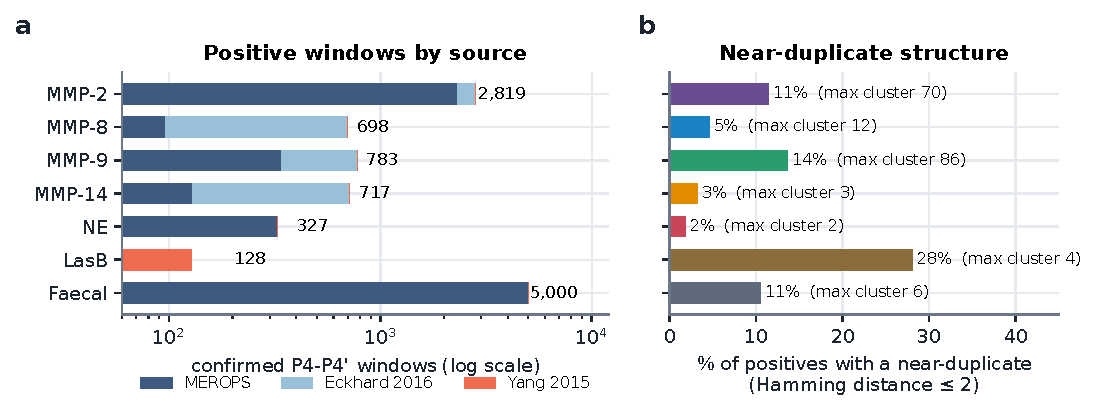
\includegraphics[width=\textwidth]{figures/F02_data_composition.pdf}
\caption{\textbf{(a)} Positive windows per protease by source (log scale). \textbf{(b)} Fraction of positives that have at least one near-duplicate (Hamming distance $\le2$) and the size of the largest cluster.}
\label{fig:data}
\end{figure}

\subsection{How different are the proteases in this data?}
Exact window overlap between protease positive sets is small (Figure~\ref{fig:sim}a; at most a Jaccard index of $0.145$, between MMP-8 and MMP-9), and windows shared with the target are removed from its negatives. But the \emph{position-specific preferences} overlap strongly among the MMPs: the PSSM log-odds vectors of MMP-2, MMP-8 and MMP-14 correlate at $r=0.73$--$0.82$, and MMP-9 correlates at $0.56$--$0.63$ with each (Figure~\ref{fig:sim}b). NE is essentially uncorrelated with the MMPs, and correlates with the faecal group at $0.46$, both being serine proteases. This structure predicts the selectivity results of Section~\ref{sec:res-sel}.

\begin{figure}[!htbp]
\centering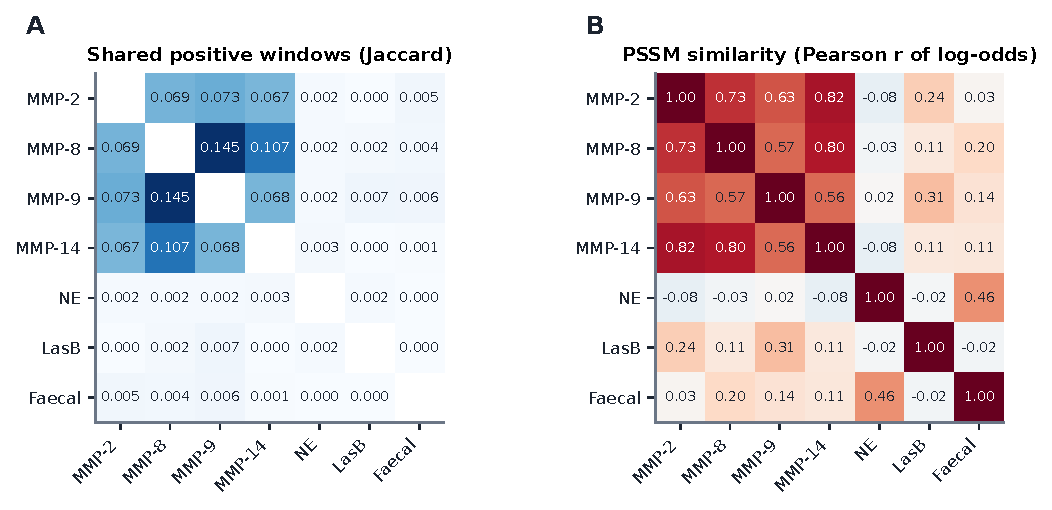
\includegraphics[width=\textwidth]{figures/F04_protease_similarity.pdf}
\caption{\textbf{(a)} Jaccard index of exact positive windows. \textbf{(b)} Pearson correlation of the $8\times20$ PSSM log-odds between protease pairs.}
\label{fig:sim}
\end{figure}

\begin{figure}[!htbp]
\centering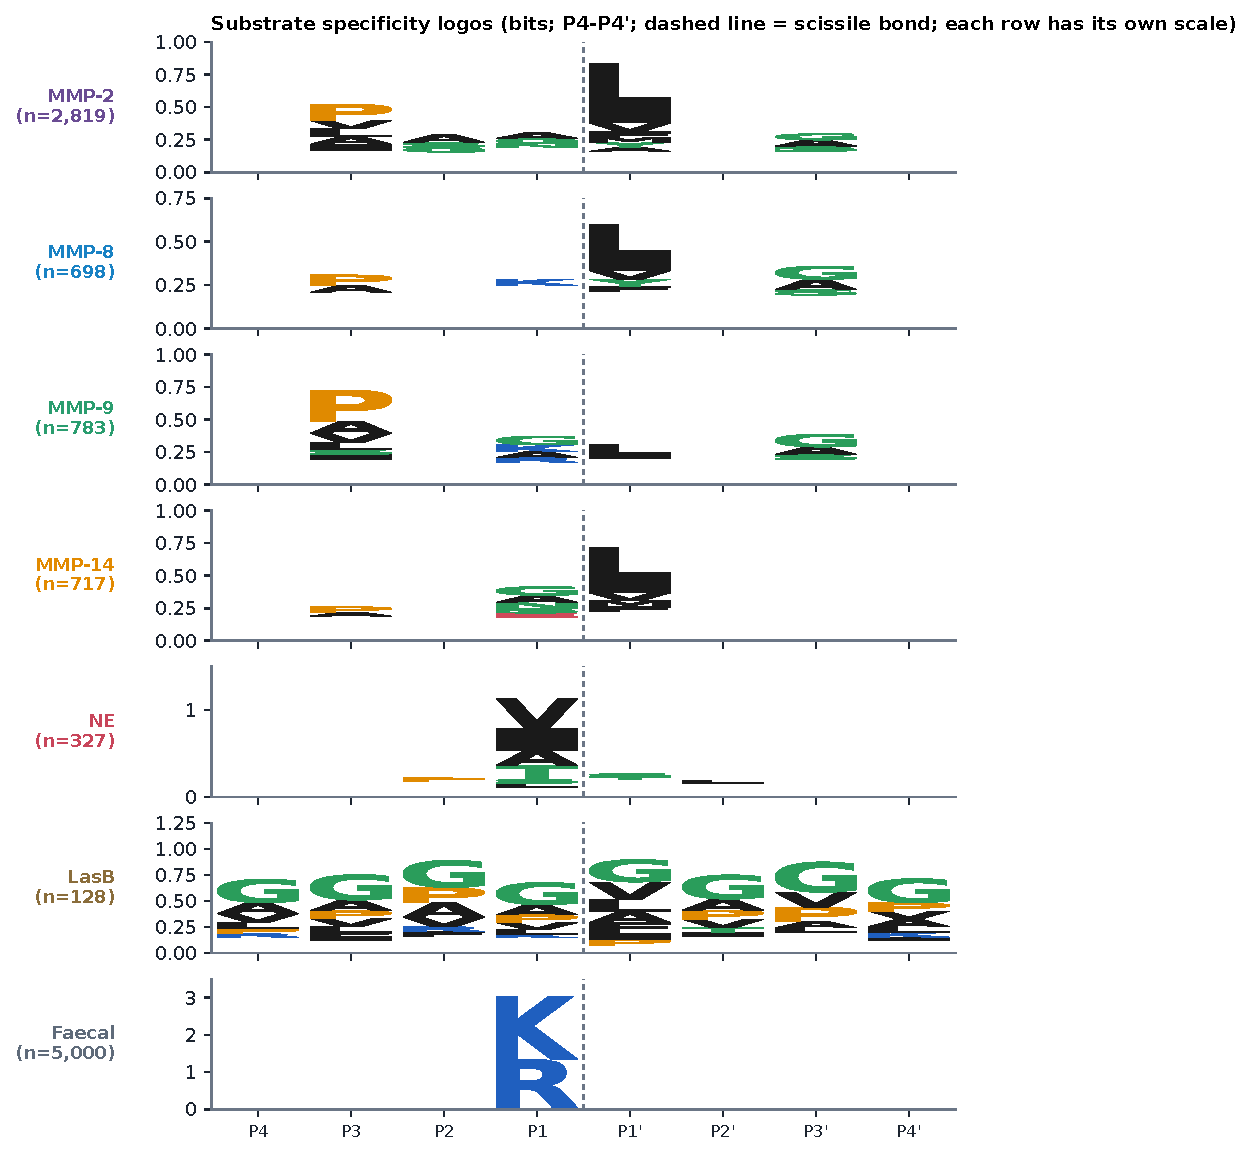
\includegraphics[width=0.86\textwidth]{figures/F03_sequence_logos.pdf}
\caption{Substrate specificity logos computed from each model's PSSM (letter height is probability times information content; each row has its own vertical scale, since the MMPs carry under one bit per position while the faecal group exceeds three at $\pos{1}$). The MMPs share Pro at $\pos{3}$ and a hydrophobic residue at $\prm{1}$; NE prefers small aliphatic residues at $\pos{1}$; the faecal group is dominated by Lys/Arg at $\pos{1}$. The LasB logo is Gly-rich because $97$ of its $128$ positives come from elastin (Section~\ref{sec:limits}).}
\label{fig:logos}
\end{figure}
